
\section{Introduction and Motivation}

Exploring long term alternatives to the CMOS technology is gaining
more and more relevance as the scaling trend of such devices keeps
introducing new challenges: power density, defect tolerance, testing
costs and wire delays are only a few of the many critical aspects
involved~\cite{itrs13}. 
While software parallelism and multicore
approaches~\cite{horowitz2004} and \cite{powell2009} are partially mitigating the impact of such
constraints on performances, it is likely that the growing computing demand will
eventually need even more radical architectural modifications and new
paradigms in order to address the Computer Design challenges of the next
decades.

In the last years, self-assembled nanoscale architectures~\cite{yan2003}
emerged as a promising technology due their tera/peta scale of
integration, defect tolerance and huge potential computing
capabilities. These technologies are certainly still at
their early stage of development, however different laboratory demos and
prof-of-concepts architectures have been presented~\cite{patwardhan2004, patwardhan2006_1, pistol2009}.
%, patwardhan2006
The main idea behind this approach is exploiting the physical regularity and
stability of DNA structures in order to create a scaffold onto which
nano-devices (e.g. nanowires and CNFETs~\cite{bachtold2001, tans1998, cui2001}) can be
attached. This can be achieved by designing appropriate complementary DNA tags for
each terminal to be placed, so that a nano device will be attached
only where its own DNA tag matches a complementary tag on the DNA grid
scaffold (see Figure~\ref{fig:nana}-a).
A detailed description of the chemical properties involved is far
beyond the scope of this paper (see also~\cite{braun1998, seeman1999}), so we will focus on
the three main challenges that this new fabrication process introduces
in Computer Design: \emph{(i) limited node complexity}, \emph{(ii) large scale
randomness} and \emph{(iii) high defect rates}.  

The \emph{limited node complexity} aspect is directly
related to the use of complementary DNA tags in order to place circuit
components. In a traditional CMOS process the complexity is introduced
using a photolithography mask, so that larger (more complex) circuits
only require larger masks; conversely, self-assembly achieves
complexity by increasing the number of unique DNA tags, since more
different tags means having more control on component placement. Ideally, by specifying a single
and unique tag for each nano transistor terminal, we could exactly
choose where each component would be placed. But the number of DNA
symbols forming the DNA sequence is limited (sequence of 4 nucleobases
G,A,T,C) and so creating many different tags (of a given length) would
mean make them more similar to each other, increasing the probability
of incorrect/partial matching. To avoid this problem we should limit
the number of unique tags, thus limiting the complexity at each node.
In particular, a budget of about $10,000$ CNFETs per node has been
estimated in~\cite{liu_jetcs}.

\emph{Large scale randomness} is the other fundamental condition of
self-assembled technology: DNA tags allow a control placement inside
node grid, but there is no control of where each of these  grids will
be placed on the whole network. As a consequence, other typical
properties of regular networks cannot be guaranteed, e.g. being
connected to a fixed number of neighbors, having a determined
orientation and so on.

Finally, \emph{defect rates}: while they are very hardly tolerated in mask
based top down design, the same nature of a bottom up self-assembly
 process cannot assume such a deterministic device placement
process, thus defect tolerance is something like a design requirement
more than an exception to be avoided.

\begin{figure*}
\centering
\begin{tabular}{cc}
    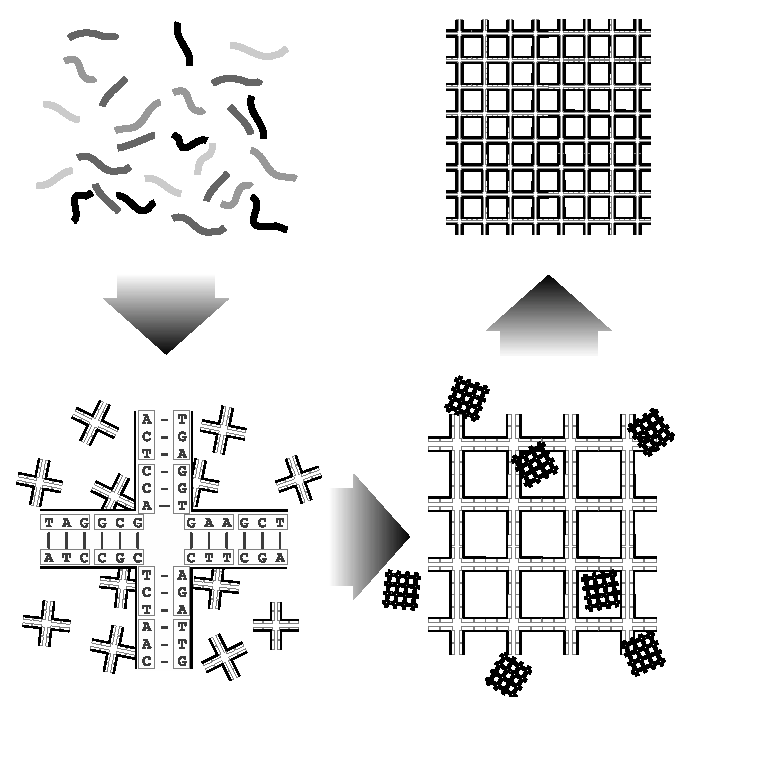
\includegraphics[width=0.40\textwidth]{pictures/dna2b.eps} &
    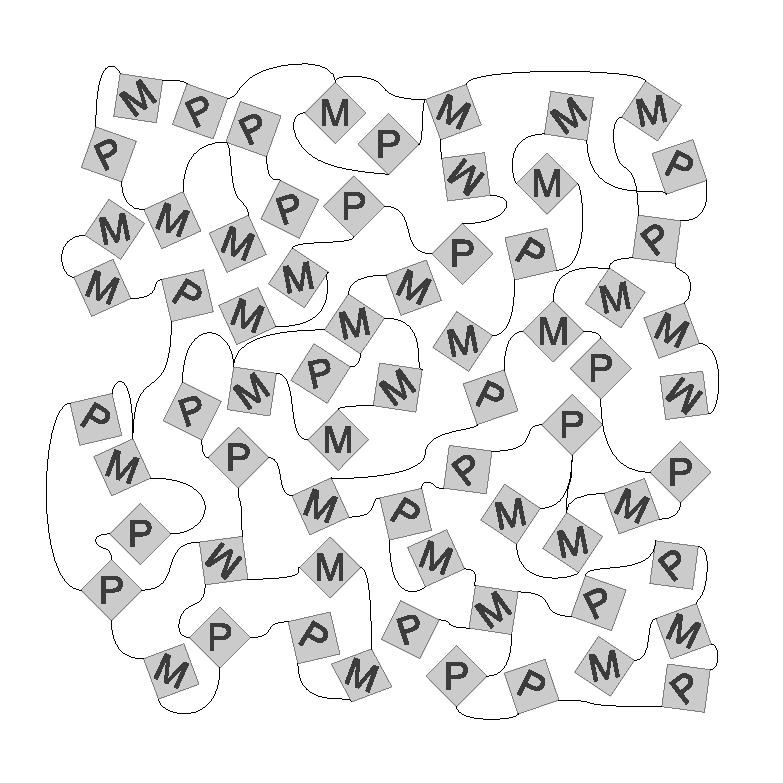
\includegraphics[width=0.40\textwidth]{pictures/dna1_complex2.eps} \\
 (a) & (b)
 \end{tabular}
  \caption{(a) DNA tag matching and (b) resulting irregular topology}
  \label{fig:nana}
\end{figure*}
These aspects of a DNA self-assembly process lead to some important
implications to be addressed when approaching to the design of
a computer architecture: computational model should be based on a
distributed network of small processing and storage nodes, randomly
placed and interconnected (see Figure~\ref{fig:nana}-b).
Proof-of-concept of such architectures can be found for
example in~\cite{patwardhan2006_1}, where instruction and data
operands are moved around the network in order to be processed.
Independently of the particular policy chosen to route packets,
such networks must be able to guarantee deadlock freedom without any
prior assumption on topology.

In this work, we introduce \disr{}, a Distributed Segment-based approach
to deadlock freedom in large scale DNA self-assembled networks. Our
contribution aims to achieve the classical properties of a
segment-based approach~\cite{mejia_ipdps06} without requiring any
topology graph, external defect map or centralized algorithm
execution.  So the \disr{} approach is not intended to discover the
``optimal'' segment choice (ideally reachable with the knowledge of
the topology graph) but just to demonstrate a concrete model that can
fit into such complex, irregular and large sized networks.
It is important to
underline that, although we can assume an architecture similar to the
one depicted in Figure~\ref{fig:nana} as background, the topology discovery
problem faced in this work is more general and not strictly dependent on any of the
underlying computing architectures.

The paper is organized as follows: in Section~\ref{sec:related_works}
we summarize the main approaches for topology agnostic routing. Next, in
Section~\ref{sec:disr_concepts} are described the main elements and
the execution model of the proposed approach. In Section~\ref{sec:simulation},
simulations are carried out with the open-source tool Nanoxim to
demonstrate how \disr{} preserves some of the main segment-based
properties and how compares to the tree-based approaches. Finally a
draft of an architectural implementation is shown in
Section~\ref{sec:implementation} to evaluate the feasibility of the
approach in terms of node complexity.

\section{Background and Contribution}
\label{sec:related_works}
Several works addressed the problem of topology agnostic deadlock
freedom introducing virtual channels~\cite{sancho2002, skeie2002,
skeie2004, koibuchi2003}, but while they show interesting
performances, the low resources available to prevent deadlocks makes them not suitable for
the DNA self-assembled networks we are assuming as
scenario.
Other topology independent algorithms~\cite{schroeder1991,
koibuchi2001, cherkasova1996} do not require any virtual channel but
exploit the concept of ``turn prohibition''.
In particular, authors of~\cite{Patwardhan05evaluatingthe} exploit the creation of a spanning tree of the
topology, placing bidirectional restrictions \hl{by avoiding a packet
to traverse the same link in both up and down directions}.
The hierarchical nature of this approach can lead to uneven traffic
distribution, with many packets traversing upper links (near to the
root), but this is quite acceptable in classical wide area networks
topologies with a limited number of nodes. Other approaches such as
FX~\cite{sancho2000} mitigate this
issue, but the set of turn restrictions is still prefixed
strictly depending on the particular tree root selected. 
Other solutions try to approach the issue of irregular
topologies by limiting the number~\cite{duato1997, gomez2004, koibuchi2008} or the
location~\cite{zhang2008, flich2008, liu2011} of missing links. This
restriction is clearly unacceptable given the hight-defect rates of
DNA self-assembled networks scenario. For the same reason, we also
avoid considering solutions based on hardware-redundancy to
dynamically recover defects as in~\cite{constantinides2006, kohler2010,  park2006, ebrahimi2013}. 

In~\cite{mejia_ipdps06} authors present an approach that solves these
limitations setting turn restrictions locally,
independently from other restrictions. The whole network is
partitioned into segments, and a bidirectional turn
restriction can be freely chosen within a segment in order to guarantee
deadlock freedom while preserving network connectivity. This \emph{locality
independence} property, removing the requirement of choosing a particular tree/root,
would make this approach the best choice for the given scenario;
however, it still requires the knowledge of the
whole network graph in order to find the segments.

The \disr{} approach presented in this work is a first attempt to
achieve the same goals of a segment based turn prohibition without
requiring neither the knowledge of a topology graph nor centralized execution. In particular
\disr{} implements segment discovery and turn prohibition using a
completely different mechanism, based on a distributed exchange of
small setup packets requiring on average $15\%$ of the available
resource budget. The following main features distinguish \disr{}
from classic approaches to segment partitioning: 
\begin{itemize}
\item No centralized entity is globally responsible and/or aware of
what is going on, i.e. the status of the \disr{} execution is
collectively distributed among the nodes
\item  No defect map and/or topology graph is used as input,
thus, the topology has to be discovered \emph{while} segments are
created
\item At the end of the execution, no segment list is created or
stored anywhere: each node is only aware of belonging to \hl{a segment | some segments},
ignoring the presence of other nodes in the same segment and also the
presence of other segments in the network
\end{itemize}


